\section{The iterative closest point (ICP) algorithm for 3D point clouds
alignment}

A common problem when performing 3D point cloud analysis is the one of finding
matches between two sets of data, each sharing a partial set of points
corresponding to a part of the scene they refer to. After finding two sets of
matches which are known to correspond each other into the scenes, the
corresponding rigid transformation between the two can be computed. If one of the two
point clouds is then transformed using this transformation, the matches will
come in (almost) exact correspondance, and the two point clouds will then refer
to the same, global coordinate system. This problem is known as
\emph{point cloud registration} or \emph{point cloud alignment}. In this case,
the point cloud which must be aligned to a fixed scene is called \emph{data
cloud}, while the fixed point cloud, set into the global reference frame, 
which the data cloud must be aligned to is called \emph{model} or
\emph{reference cloud}.

If the scene is known to be still, this can be used to assemble together
different views of a same scene,
taken from different positions either by purpose or due to human error; in
fact, one of the most common use of registration algorithms is 3D scene
reconstruction starting from a set of views of the same scene. This is useful
for example in 3D scanning applications, where a 3D camera (like a Microsoft
Kinect) is moved slowly around an object and subsequent shots are taken;
after doing this, each image is registered to the previous one and a
bigger and bigger point cloud is obtained each time. When the last image is
reached, it is aligned to a known, ground-truth location to obtain a full
reconstruction of the scanned object in 3D global coordinates.

In this project, point cloud registration is used to find a transformation
between a computer-generated image -- the render of an object which is thought
to be recognized into the world -- and the real scene to which the image refers
to, i.e. the portion of image in which the object is thought to have been
found. The practical effect of this is that, if the object which will be
aligned to the scene is rendered with an associated, known pose, by applying
the resulting transformation the correct, refined pose of the object in the 3D
space can be found. This will be used in the later stages of the execution by
the gripper's algorithm.

Although numerous algorithms have been developed for 3D point clouds
registration, one of the most known and used ones remain the
\emph{Iterative Closest Point (\emph{ICP})}. Introduced first in 1992 in
\cite{icp}, the algorithm had sudden success into the computer vision
environment, due to its extreme simplicity, low computational cost and high
effectiveness. Numerous variants have been developed, which target either
computational efficiency, such the ones described in
\cite{icp-fast-algorithms}, or robustness with respect to certain parameters,
such as measurement noise, as in \cite{icp-bayes}, or a good compromise between the
two as in \cite{icp-robust}. The basic concept between these implementation
remains, anyway, always the same, and thus the processing steps stated in
\cite{icp} are taken here as a reference.

ICP is based on the assumption that, given a set of points with a good starting
guess for their reciprocal transformation, the point which corresponds to a
datum point into the data cloud is the one which is its
nearest neighbour in the reference cloud. At each instant within the
algorithm, a rough estimation of the transformation can be defined by computing
the transformation that would minimize the average distance between these
points. If the whole data cloud is then transformed using this transformation,
it will come closer to the reference; by iterating these steps several times a
solution can be found.

\subsection{Closest point computation}
First of all, the notion of \emph{distance} $d(\vec{p},C)$ between a point $\vec{p}$ in the data cloud
and a given model $C$ -- composed of $N_c$ model points $\vec{m_i}, i \in \{0 \dots
N_c\}$  -- is introduced:

\begin{equation}
  d(\vec{p},C) = \text{min}\left\{ E(\vec{p}, \vec{m}) : \vec{m} \in C \right\}
\end{equation}

Here, $E(\vec{x},\vec{y})=\lVert \vec{x} - \vec{y} \rVert$ represents the well-known
euclidean distance between two points. With this definition, the distance of a
point $\vec{p}$ to a cloud is given as the distance from $p$ to its closest
point within $C$. Using the same definition, the closest point $\vec{p_c}$ to
$\vec{p}$ is the point satisfying the equation $E(\vec{p},
\vec{p_c})=d(\vec{p}, C)$. Finding this point is an operation which can be done
with an average cost of $O\left(\text{log}\left(N_c\right)\right)$ using a K-D
tree as explained in sec. \ref{kdtree}, and with a worst-case computational cost of
$O\left( N_c \right)$; thus, finding the complete set of closest points to
every point in the reference, i.e. finding the set $P_{c} = \left\{ p_c :
E(\vec{p},\vec{p_c}) = d(\vec{p},C) , p \in C \right\}$, has an average
computational time of $O\left( N_p \text{log}\left(N_c\right) \right)$, and a
worst-case one of $O\left( N_p N_c \right)$.

\subsection{Best transformation choice} \label{sec:icp-best-transformation}
After assigning to each point in the data cloud a correspondance within the
model cloud, the problem of finding the best transformation, which is the one
giving the least possible average squared distance between every point $p$ and
its corresponding point $p_c$, has two well-known solutions. 

In the case of 3D point clouds with no additional informations to register, a
good approach is the use of unit quaternions, i.e. quaternions $q$ which norm is
equal to 1:

\begin{equation} \label{eqn:quaternion}
q = \begin{pmatrix}a\\b\\c\\d\end{pmatrix}, a^2+b^2+c^2+d^2=1
\end{equation}

Unit quaternions are a well-known form of representation for rotations, which can
thus be combined with a translation to form a complete affine transformation
representing reciprocal pose\footnote{In this case, the scaling factor $s$ of
  the resulting affine transformation is assumed to be 1, as the registration is
  performed between clouds of the same scale (i.e. the registration process
results in a rigid transformation)}. Given the quaternion $q$ of
eqn.\ref{eqn:quaternion}, it can be univocally associated with a rotation
matrix, without redundancy:

\begin{equation}
  R = \begin{pmatrix}
    a^2+b^2-c^2-d^3 & 2\left(b c - a d \right) & 2\left( b d + a c \right) \\
    2\left(b c + a d \right) & a^2+c^2-b^2-d^2 & 2\left( c d - a b \right) \\
    2\left( b d - a c \right) & 2\left(c d + a b\right) & a^2+d^2-b^2-c^2
  \end{pmatrix}
\end{equation}

If a translation vector $t=\begin{pmatrix}x_0 & y_0 & z_0\end{pmatrix}^{\tau}$
is combined with $R$, and this affine transformation is applied to the point
$p$, the resulting point $p_1$ will be:
\begin{equation}
  p_1=R*p+t
\end{equation}

Thus, in order to find the optimal transformation between the two clouds, $R$
and $t$ must be found so that

\begin{equation}
  S=\frac{1}{N_p}\sum_{i=1}^{N_p}\lVert p_{c,i} - Rp_i -t  \rVert
\end{equation}

is minimized.

It has been proven in \cite{extrinsics-algorithm}that the optimal rotation
quaternion $q$ can be found by first computing the centers of mass of the data
cloud $\vec{\mu_d}$ and of the reference cloud $\vec{\mu_r}$, then using these for
computing the cross-covariance matrix $\Sigma_{p}$ between the two points' set:

\begin{eqnarray}
  \vec{\mu_d} & = &  \frac{1}{N_p}\sum_{i=1}^{N_p}\left(\vec{p_i}\right) \\
  \vec{\mu_r} & = &  \frac{1}{N_p}\sum_{i=1}^{N_p}\left(\vec{p_{c,i}}\right) \\
  \Sigma_{p} & = &
  \frac{1}{N_p}\sum_{i=1}^{N_p}\left[\left(\vec{p_i}-\vec{\mu_d}\right)\left(\vec{p_{c,i}}-\vec{\mu_r}\right)\right]
\end{eqnarray}

After this, the matrix $A=\Sigma_{p}-\Sigma_{p}^{\tau}$ is built, and its cyclic
components are used to build a column vector $\Delta$. These data are used to
build the $4 \times 4$ matrix $Q$ shown in
eqn.\ref{eqn:q-of-extrinsics-algorithm}, and the best solution for $q$ is given
by the eigenvector of $Q$ corresponding to its maximum eigenvalue.

\begin{eqnarray}
  A & = & \Sigma_{p}-\Sigma{p}^{\tau} \\
\Delta & = & \begin{pmatrix}A_{2,3}\\A_{3,1}\\A_{1,2}\end{pmatrix} \\
  Q & = & \begin{pmatrix}
  \text{tr}(\Sigma_{p}) & \Delta T \\
  \Delta & \Sigma_{p}+\Sigma_{p}^{\tau}-\text{tr}(\Sigma_{p}I_{3}) 
\end{pmatrix} \label{eqn:q-of-extrinsics-algorithm}\\
q & = & \left\{ \vec{x} \in \text{Eigenvectors}(Q) :
  \text{Eigenvalue}(x)=\text{max}\left(\text{Eigenvalue}(x)\right) \right\}
\end{eqnarray}


After finding the rotation matrix $R$ as described above, it has been shown that the best solution for $t$
is for it to be the translation vector between the center of mass of the
reference cloud $\vec{M_{r}}$ and the one of the rotated
data cloud $R\vec{M_d}$ 

\begin{equation}
  t = \vec{M_r}-R\vec{M_d} =  \frac{1}{N_p}\sum_{i=1}^{N_p}\left(\vec{p_{c,i}}-R\vec{p_{i}}\right) 
\end{equation}

With this procedure, best transformation between corresponding point clouds can
be found in $O(N_p)$ steps.

\subsection{Iterations and ending conditions}
The ICP algorithm applies the two previous steps of nearest neighbour search and
best transformation computation iteratively, hence its name; at every step, the
relative pose between the two clouds gets better. This is not only an heuristic
supposition, as a theorem has been proven
proven in \cite{icp}, stating that the whole algorithm will converge
\emph{monotonically} to a minimum of the distance function: thus, every
iteration will yield to a better result no matter the current state of the
algorithm.

Two main termination conditions are used by ICP: the first is the best-case one,
in which the total distance between the two point clouds $R$ and $D$ becomes smaller than a
given threshold:
\begin{equation}
  d(D,R) = \sum_{i=1}^{N_p}\left(p_i,R\right) < t_{\text{good}}
\end{equation}

The second is a condition that lets the algorithm end if it is stuck in a local
minimum of the distance function: in this case, as the error will always
decrease as stated before, its variation will decrease too and eventually become
smaller than a certain threshold $t_{\text{stop}}$ at time $t$:
\begin{equation}
  \Delta d_t(D,R) = d_t(D,R)-d_t(D,R) < t_{\text{stop}}
\end{equation}

The whole algorithm can be then summed up in this way:
\begin{enumerate}
\item{Start with given data cloud $D$, reference cloud $R$, transformation
  guess $P$, last transformation $T=P$;}
\item{Transform each point $p \in D$ using the current transformation $T$;}
\item{For each point, search for the nearest neighbour $p_c \in R$ and create
  the set of associations $A=\left\{(p,p_c) : p \in D \right\}$;}
\item{Find the best transformation from $D$ to $A$ as explained in sec.
  \ref{sec:icp-best-transformation}, and save it into $T$;}
\item{Stack the current transformations together into $P$: $P=TP$;}
\item{If $d(D,R)<t_{\text{good}}$ or $\Delta d(D,R)<t_{\text{stop}}$, exit;}
\item{Go to step 2.}
\end{enumerate}
\subsection{$K$-d Trees} \label{kdtree}
In order for the problem of finding the closest point $\vec{p_c}$ to $p$ not to
have fixed computational cost $O(n)$, a \emph{$K$-d tree} (i.e.
$K$-dimension tree) is used; it is
a data structure which extends to more than one dimension the concept of binary
partition tree. If a point cloud is organized using a $K$-d tree, its points
result iteratively sorted with respect to their coordinates, which allows a
faster division of the search space.

As in a binary tree, data inserted in a $K$-d tree is organized in a
hierarchical way. Each item in the tree is a single vector with $K$ dimensions.
Starting from the top node, called \emph{root}, navigation into the tree is done
top-down: nodes have two trees below them (called \emph{subtrees}), containing one
or more elements, called \emph{children}; children in the first (or \emph{left})
subtree are always lesser then their father's node, with respect to a certain
evaluation function, while children in the second (\emph{right}) subtree are
greater\footnote{The case in which an exact duplicate of a datum is inserted is
 not covered here, as it is assumed that the point cloud to be transformed in a
 $K$-d tree is sparse enough.}. The discriminant function for a given node is usually chosen to be an hyperplane, to
which the node belongs to: in
this way, the whole points' space is, at each level, subdivided in half. Thus,
points which belong to the same subtree are spatially near each other.
Fig.~\ref{fig:kd-tree-subdiv} exemplifies this concept.

For 3D data, the choice of the hyperplane can be different at each level of
subdivision: the dividing plane is usually chosen to be parallel to the X axis
for the first level, Y axis for the third level, and so on; this makes the
discriminant function very lightweight, as it only consists of comparing one of
the coordinates of the object to be inserted (or searched for) with the same
coordinate of the current node.

\begin{figure}[htbp]
\centering
  \includegraphics[width=2.5in]{./Graphics/kdtree} 
  \caption{A $K$-d tree recursively subdivides the data space in smaller
  hypercubes by means of hyperplanes: thus, points belonging to the same subtree
  are spatially near to each
  other. Image source:
https://upload.wikimedia.org/wikipedia/commons/b/b6/3dtree.png (GNU GPLv2)  \label{fig:kd-tree-subdiv}}
\end{figure}

If a new value must be inserted into a list, the usual rules of BSTs apply:
the value is compared with the root node, and the insertion algorithm moves to
the left or to the right subtree based on the result of this comparison. This
process is reiterated, and the
value is inserted when the algorithm reaches a node which has no subtree into
which to move further (\emph{leaf}). The problem with this approach is the
possibility of building a tree which is not \emph{balanced}, i.e. with a much
higher number of nodes in one of the subtrees with respect to the other. However,
when building a $K$-d tree out of a point list, the insertion algorithm can sort
the elements to be added before starting: in this way, a balanced tree is easier
to build, as it is sufficient to choose, for each subtree, the median element of
the data as the root.

When the whole tree has been built, it is easy to exploit its properties to
simplify the operation of nearest-neighbour search for a datum value. The
algorithm is recursive, and proceeds by searching the nearest neighbour in one
of the subtrees, then exploiting the properties of $K$-d trees to avoid
computation on the other subtree if not strictly necessary. In practice, given
the point $\vec{P}=\left(p_0,p_1,\dots,p_n\right)$, it goes
as follows:

\begin{enumerate}
  \item{At start, set the distance of the nearest neighbour to be $d=+\infty$
    and the root of the tree as the current node;}
  \item{the nearest neighbour is the root node if the tree has only 1 element
    (termination condition);}
  \item{if the current node $\vec{C}=\left(c_0,c_1,\dots,c_n\right)$ has a lower distance than the best one, set it as
    the nearest neighbour;}
  \item{search the nearest neighbour (recursion step) into the tree $T_1$ to which $\vec{P}$
      belongs to, i.e. into the left tree if $p_i < c_i$, into the right tree
    otherwise; update $d$ if a new nearest neighbour has been found;}
  \item{using the current best distance, examine whether the other branch $T_2$ of
      the tree has to be examined. This is the \emph{crucial} step of the
      algorithm, being the one that makes it better with respect to the trivial
    ones. Geometrically, the other branch of the tree must not be examined if no
    point lies on the other half of the space such that it is contained in the
    hypersphere centered in $\vec{P}$ and with radius $d$; however, for how the $K$-d
    tree is structured, it can be seen that this definition is equivalent to
    saying that the same sphere does not cross the division hyperplane generated
    by $\vec{C}$: this, in turn, is equivalent to saying that the distance from $\vec{P}$
    and $\vec{C}$ (taking only the $i$-th coordinate into account) is less than $d$:
    \begin{equation}
      \not \exists \vec{x} \in T_2 : \lVert \vec{x}-\vec{P} \rVert < d
      \Leftrightarrow \lvert c_i-p_i \rvert < d
    \end{equation}
    if this property, which is shown in fig. \ref{fig:kdtree-hypersphere}, does not apply, search recursively into the other branch
  $T_2$ as well.}
\end{enumerate}

\begin{figure}[htbp]
\centering
  \adjustbox{valign=m}{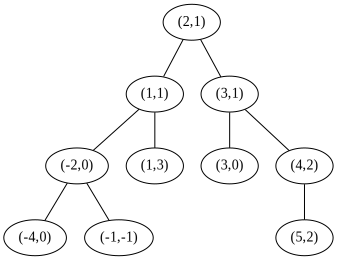
\includegraphics[width=2in]{./Graphics/kdtree_graph}} 
  \vspace{0.5in}
\begin{tabular}{c|c}
  \adjustbox{valign=m}{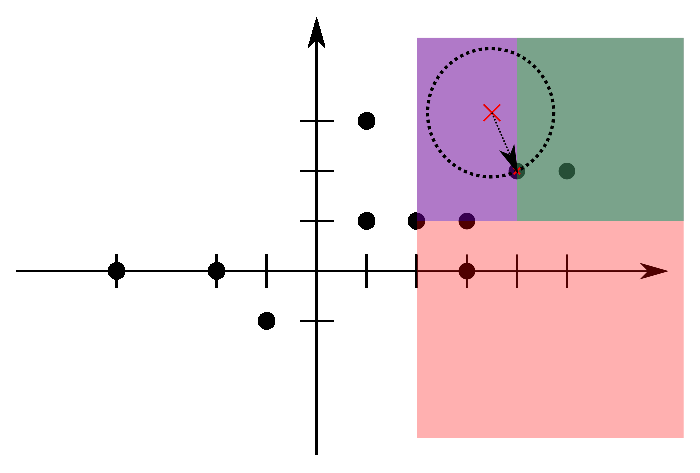
\includegraphics[width=2in]{./Graphics/kdtree_plane_2}} &
  \adjustbox{valign=m}{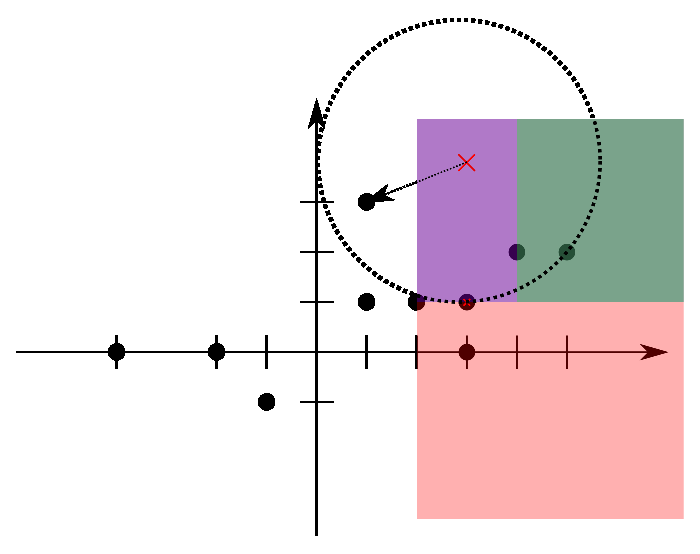
\includegraphics[width=2in]{./Graphics/kdtree_plane_1}}
\end{tabular}
    \caption{A $K$-d tree, like the one shown on the top, subdivides the
      points' space based on points' coordinates. If the distance from a point
      $\vec{P}$
      to an hyperplane is less than a value $d$, then no points on the other
      half of the space have a distance smaller than $d$ to $\vec{P}$ (left). If
      there is such a point, the distance from the point to the plane is smaller
    than $d$ too: this means that the hypersphere centered in $\vec{P}$ of
  radius $d$ crosses the plane (right). \label{fig:kdtree-hypersphere}} 
\end{figure}

Exact computational analysis of this algorithm is quite tricky; however, it is
intuitive to see that, given a well-balanced $K$-d tree and a point chosen
randomly, the algorithm will skip processing half of the tree about one half of
the times: this gives an average  execution time of $O(\log N_p)$, as stated
before.

